\section*{はじめに}
本ドキュメントは、ユーザーランドで動作するGfarm ファイルシステムを
カーネル内FSから直接呼び出すことによって性能向上を図るための
カーネルドライバの仕様を記述するものである。

\section{システム概要}

以下に本システムのモジュール関連図を示す。

\begin{figure}[htb]\begin{center}
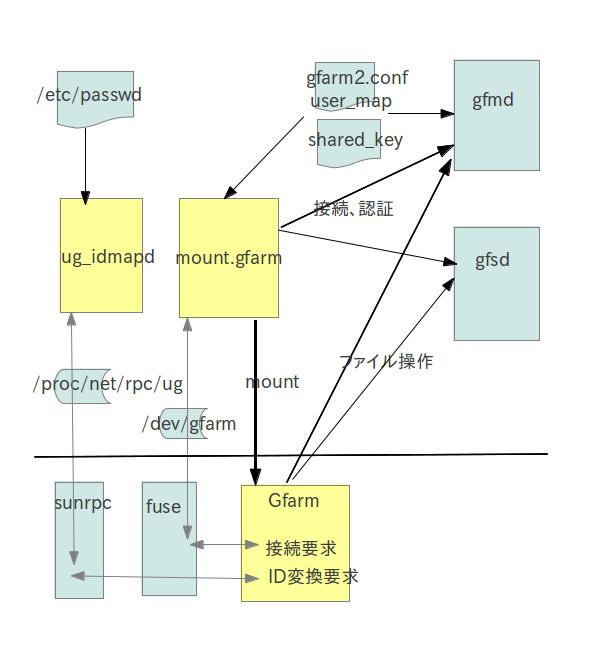
\includegraphics[bb=00 00 800 850,scale=0.5]{module.jpg}
\caption{モジュール関連図}\label{fig:module}
\end{center}\end{figure}

Gfarm では各種認証機構をサポートしているが、カーネル内で認証ライブラリを
利用するのが難しいことから、今回開発では認証はユーザーランドで行う。
将来は、簡単な認証機構を導入するなどして、カーネル内に閉じて接続を
行うことも考えられる。但し、その場合も名前解決などはユーザーランドで
行うことになる。

認証はユーザー毎に行うので、サーバーとの接続もユーザー毎に行う。
同一ユーザーで複数の接続を行うことも考えられるが、ポート数の問題なども
あり、今回はユーザ毎に一つの接続とする。

今回開発するモジュールとしては以下のものがある。
\begin{itemize}
\item	gfarm \par
	カーネル内ファイルシステム。
	
\item	mount.gfarm \par
	ユーザーランドのヘルパーデーモンで、
	mount コマンドから起動される。
	mount 後はカーネルからの接続要求を待ち受け、メタデータサーバに
	接続し、認証を行う。
\item	ug_idmapd \par
	ユーザーランドのヘルパーデーモンで、
	ユーザーID、グループIDおよびホスト名の変換を行う。
\end{itemize}

ユーザーランドとの通信方法については、以下の方式とする。
\begin{itemize}
\item	接続要求	\par
	カーネルドライバが、メタデータサーバとの接続を依頼する
	インタフェースには、character device を利用する。

	これは、アプリケーションが /dev/gfarm をオープンし、
	このファイルを読み込むことによって、カーネルモジュールの
	要求を得、ユーザー空間でこれを解決して、当該ファイルに応答を
	書き込む仕組みである。

	ファイルとファイルシステムを結びつける方法は、
	アプリケーションがオープンファイルデスクリプタを
	mount時に通知することで行う。
	
	この方法は、mountと結びついて安全であるが、他方、アプリケーションが
	異常終了した際の救済手段を別途考える必要がある。

	接続要求は将来開発でなくなるので、救済手段は講じない。

\item	ID変換要求	\par
	カーネルドライバが、uid, gid と名前の変換を依頼するインタフェースには
	sunrpc モジュールがエクスポートしているインタフェースを利用する。

	これは、アプリケーションが /proc/net/rpc/配下のファイルをオープンし、
	このファイルを読み込むことによって、カーネルモジュールの
	要求を得、ユーザー空間でこれを解決して、当該ファイルに応答を
	書き込むととに、sunrpcモジュールがキャッシュ機構を提供し、
	要求応答を一定期間キャッシュし、この検索再利用を可能とさせる
	仕組みである。
	
	本システムでは、以下のインタフェースを作成する。
	\begin{itembox}[l]{/proc}\begin{cprog}
	/proc/net/rpc/ug.idtoname:	UID,GID から名前への変換
			   channel	要求チャネル
			   content	キャッシュ情報
			   flush	キャッシュフラッシュ指示

	/proc/net/rpc/ug.nametoid:	名前からUID,GID への変換
			   channel
			   content
			   flush

	/proc/net/rpc/ug.hostname:	ホスト名からIPアドレスへの変換
			   channel
			   content
			   flush
	\end{cprog}\end{itembox}

\end{itemize}

\section{mount}

mount は メタデータサーバ毎に行う。同一のメタデータサーバーへの
複数のmount は特に禁じない。

mount は ユーザーランドでメタデータサーバーとの接続を確認した上で、
mountシステムコールを発行するので、接続するユーザーを指定したmount となる。

\subsection{mount.gfarm}
	mount.gfarm はmount コマンドから
	mount -t gfarm を指定された時に呼び出される。

	オプションは以下のものがある。
	\begin{itemize}
	\item	luser=name	\par
		メタデータサーバとの接続を行うユーザーのローカルユーザ名。
		指定されなければローカルユーザIDから得る。
	\item	uid=uid	\par
		メタデータサーバとの接続を行うユーザーのローカルユーザID。
		指定されなければローカルユーザ名から得る。
		得られれなければ実行ユーザーIDから得る
	\item	key_path=path	\par
		共通鍵方式の鍵ファイルのパスを指定する。
		指定されなければluser のホームディレクトリの鍵ファイルを
		参照する。
	\item	conf_path=path	\par
		コンフィグレーションファイルのパスを指定する。
		指定されなければluser のホームディレクトリのファイルを
		参照する。
	\end{itemize}

	mount の一般的なオプションも受け入れるが、動作はメタデータサーバに
	依存する。

\paragraph{gfarm2_conf に追加されたオプション} には以下のものがある。
	\begin{itemize}
	\item	page_cache_timeout	\par
		ページキャッシュの保持ミリ秒で、デフォルトは1秒である。
	\end{itemize}

\paragraph{mount.gfarm} のmount 動作概要

	\begin{enumerate}
	\item	コンフィグレーションファイルを読み込む。
	\item	指定されたユーザーでメタデータサーバに接続する。
	\item	認証を済ませる。
	\item	/dev/gfarm をオープンする。
	\item	接続デスクリプタとデバイスデスクリプタをmount引数に加える。
	\item	コンフィグレーションファイルとグローバル名変換ファイルを
		読み込み、mount引数に加える。
	\item	mount システムコールを発行する。
	\item	/etc/mtab に登録する。
	\item	接続要求待ちループに入る。
	\item	/dev/gfarm から接続要求があればforkする。
	\item	fork した子
		\begin{enumerate}
		\item	指定ユーザーのための接続を行う。
		\item	認証を行う。
		\item	ファイルデスクリプタを /dev/gfarm に書き込む
		\item	終了する。
		\end{enumerate}
	\item	/dev/gfarm から終了を読み込んだら終了する。
	\end{enumerate}

\subsection{gfsk_mount_data}

	mount のためのオプションはバイナリデータとする。

	\begin{itembox}[l]{gfsk_mount_data}\begin{cprog}
         struct gfsk_strdata {
                int     d_len;
                char    *d_buf;
        };
        struct gfsk_fbuf {
                struct gfsk_strdata f_name;             /* file name */
                struct gfsk_strdata f_buf;              /* file content */
        };

        #define GFSK_VER1       0x30313031
        #define GFSK_VER        GFSK_VER1
        struct gfsk_mount_data {
                int     m_version;
                char    m_fsid[8];                 /* out: file system id */
                struct gfsk_fbuf m_fbuf[GFSK_FBUF_MAX];
                int     m_dfd;                     /* dev fd */
                uid_t   m_uid;
                char    m_uidname[GFSK_MAX_USERNAME_LEN];
                int     m_mfd;                     /* meta sever fd */
                char    m_host[MAXHOSTNAMELEN];    /* connected host by m_fd */
                int     m_optlen;
                char    m_opt[1];                  /* option string */
        };
        #define GFSK_OPTLEN_MAX (PAGE_SIZE - sizeof(struct gfsk_mount_data))
	\end{cprog}\end{itembox}

	\begin{itemize}
	\item	m_fbuf はコンフィグレーションファイル、グローバル名変換ファイル
		などをmmap してカーネルに内容を通知するための構造である。

		カーネル空間を圧迫する恐れがあるので望ましくないが、
		今後の検討課題とする。
	\item	m_dfd は /dev/gfarm を開いたファイルデスクリプタで、
		カーネルからの接続要求を受け付けるためのものである。
	\item	m_mfd は メタデータサーバに接続したファイルデスクリプタで
		カーネルに引き渡すものである。
	\item	m_uid,m_uidnameはメタデータサーバに接続したユーザー情報である。
	\item	m_hostは接続したメタデータサーバである。
	\item	m_optは一般的な mount オプション文字列である。
	\end{itemize}
\subsection{gfarmfs}

\paragraph{Gfarm カーネルドライバ版} のmount 動作概要
	\begin{enumerate}
	\item	module ロード時	\par
		\begin{enumerate}
		\item	modprobe のオプションで設定パラメタを渡される。
			設定パラメタは以下である。
			\begin{itemize}
			\item ug_timeout_sec=N	\par
				ug_idmapd からの応答待ち時間を設定する。
				デフォルトは1秒である。
			\item gflog_level=N	\par
				ログレベルを指定する。
				0はログが少なく7は多い。
				ただし、後のmount で上書きされる。
			\end{itemize}
		\item	register_filesystem(file_system_type) で
			get_sb, kill_sb 関数を登録する。
		\item	/dev/gfarm の登録を行う。
		\item	ug_idmapd のための登録を行う。
		\end{enumerate}
	\item	mount 時
		\begin{enumerate}
		\item	mount.gfarm からmount システムコールが発行される。
		\item	マウントオプションをチェックする。	\par
		
			mount は複数可能とする。
			ただし、今期試験は単数のみとする。

			mount の単位は本来 メタサーバ(グループ)毎
			かもしれないが、nfs 同様、特にチェックはしない。
			
		\item	ファイルシステム固有データ構造を初期化する。
		\item	コンフィグレーションファイルに従い初期化する。
		\item	渡された接続fdでサーバーからroot ディレクトリ情報を
			得る。
		\item	fill_super でfs情報を得る。
		\end{enumerate}
	\end{enumerate}


\subsection{umount}
	MNT_DETACH はサポートしない。
	MNT_FORCE が指定されたら通信中のプロセスは起こしEIOで戻す。

	umount 時は gfskd に通知した上、
	gfskdの file struct の private メンバ(gfarm_fsctx を指している) を
	クリアし、以降のread を失敗させる。

\section{データ構造}

\subsection{ 外部変数閉じ込め }

	既存のGfarm で外部変数となっていて、mount 毎に保持する必要の
	あるものは struct gfarm_context に閉じ込める。
	現在ローカルに定義されている構造体については、
	ポインターメンバーとして、各初期化時にアロケートし、
	gfarm_context からポイントする。


	gfarm_context を
	関数引数として連れ回すのは大変なので、task コンテクストから
	とれるようにする。
	struct task の journal_info がファイルシステムでテンポラリに
	利用可能なので、これを利用する。

	\begin{itembox}[l]{gfarm_context}\begin{cprog}
        struct gfarm_context {
                /* global variables in config.c */
                char *metadb_server_name;
                int metadb_server_port;
                char *metadb_admin_user;
                char *metadb_admin_user_gsi_dn;
		.....
        };
        #ifdef __KERNEL__
        #define gfarm_ctxp (gfsk_task_ctxp->gk_gfarm_ctxp)
        #define errno        gfarm_ctxp->gc_errno
        #else
        extern struct gfarm_context  *gfarm_ctxp;
        #endif
	\end{cprog}\end{itembox}

	カーネル内では各システムコールの入り口となる関数で、
	gfsk_task_contextをスタックに作成し、current task に設定し、
	戻りでクリアする。

	但し、ローカルファイルシステムを呼び出すときはクリアしなおす。


\subsection{ファイルシステムデータ構造}
	linux のファイルシステム関連のデータには以下のものがある。
	\begin{enumerate}
	\item	struct super_block \par
		マウント毎のファイルシステム情報。

		fs 用の void *s_fs_info がある。	
	\item	struct dentry \par
		ディレクトリキャッシュでネガティブキャッシュもある。
		lookup で 作成し、inode_operations.lookup に渡して、
		inode を結びつけさせる。
		
		fs 用の void *d_fsdata がある。	
	\item	struct inode \par
		inode_operations.lookup で dentry に結びつける時に fsで
		作成する。
		dentry を解放するdentry_iput 時にinodeがあれば、
		d_iput が定義されていれば呼びだす、inode 解放は fs に任される。
		d_iput が定義されていなければ inode の参照数を落とし、0なら
		drop_inodeが定義されていれば削除を任せる。
		

		fs 用の void *i_private もあるが、fs 固有inode に
                含ませる実装も多い。
	\item	struct file \par
		ファイルのオープンコンテクストで、
		ファイルオープン時、作成後 file_operations.open を呼び出す。
		最後のクローズ時、file_operations.release を呼び出す。

		fs 用の void *private_data がある。	

	\item	struct vm_area_struct \par
		仮想アドレススペースのメモリとファイルの定義を行う。
		ここの vm_file はメモリをマップしているファイルである。
	\end{enumerate}
\clearpage

\begin{figure}[htb]\begin{center}
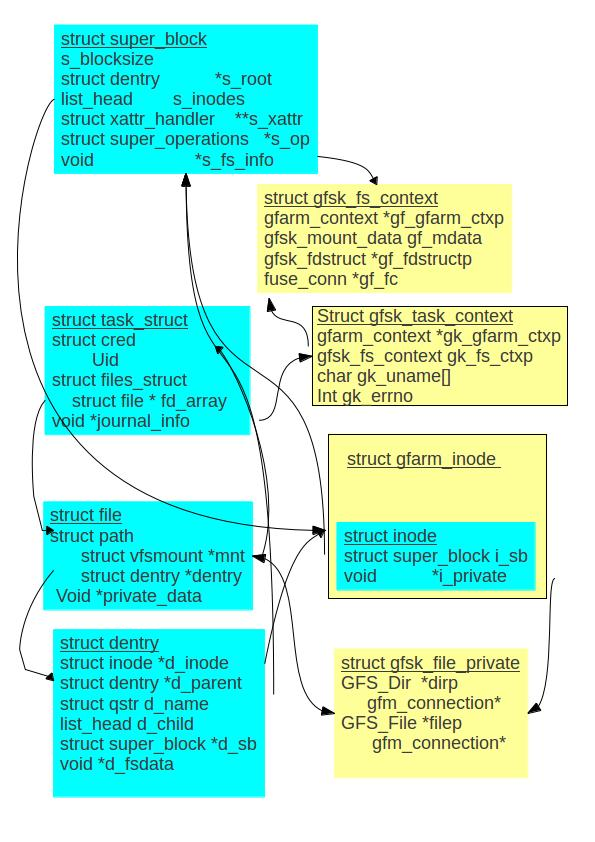
\includegraphics[bb=00 00 800 1000,scale=0.5]{fsdata.jpg}
\caption{データ構造関連図}\label{fig:data}
\end{center}\end{figure}

各linux のデータ構造に対応して図 \ref{fig:data} のように固有のデータ構造を
つくる。

	\begin{itemize}
	\item	gfsk_fs_context	\par
		カーネルドライバ固有ファイルシステム情報
		\begin{itemize}
		\item	struct gfsk_mount_data  gf_mdata	\par
			mount 引数をカーネル内で保持する。
			コンフィグレーションファイルもここからマップされる。
		\item	struct gfarm_context    *gf_gfarm_ctxp	\par
			Gfarm fs の外部変数を閉じ込めたfs毎のデータ。
		\item	struct gfsk_fdstruct    *gf_fdstructp	\par
			ファイルデスクリプタを struct file ではなく、
			int で受け渡すための管理データ。
		\item	struct gfskdev_conn        *gf_dc	\par
			mount.gfarm に依頼するためのインタフェースコンテクスト。
		\end{itemize}

		ユーザーIDからサーバー接続情報を探すためのリストは、
		gfm_server_cache にユーザー名があるので、 これを利用する。

        \item	struct gfsk_task_context \par
		current task に結びつけるコンテクスト情報で、ファイルシステム
		IFに入ったときに設定し、関数から出るときにクリアする。

		\begin{itemize}
		\item	struct gfsk_fs_context *gk_fs_ctxp \par
			操作中のファイルシステム。
		\item	char    gk_uname[GFSK_USERNAME_MAX] \par
			当該タスクのユーザー名キャッシュ。
		\item	int gk_errno \par
			Gfarm ライブラリ内で参照される errno データ。
		\end{itemize}
        \item	struct gfarm_inode \par

		\begin{itemize}
		\item	struct inode         inode \par

		inode 管理は vfs 層のinode 管理を利用する。

		linux では inode の作成は ファイルシステムが用意していれば
		それを、そうでなければ inode_cache から作成する。

		さらに、ino をファイル識別に用いるファイルシステムのために
		ino によるinode 管理も提供しており、iget_locked で探索、
		作成を行える。

		Gfarm では inum, igen が用意されているので、inum を
		利用する。 igen はファイルシステム内でチェックし、
		更新されていれば古いファイルを捨てる処理を行う。

		コンパウンド要求の途中で得られたのみの情報でも inode を
		作成する。
		\item	uint64_t        i_gen	\par
			vfs inode に持てない i_gen 情報。
		\item	uint64_t	i_actime	\par
			属性キャッシュの保持時間
		\item	uint64_t	i_pctime	\par
			ページキャッシュの保持時間
		\item	struct list_head i_openfile	\par
			ダーティページフラッシュに備えるための、
			write オープンしているファイルのリスト。
		\item	int		i_wopencnt	\par
			write オープンしているファイルの数。
		\item	loff_t          i_direntsize	\par
			ページキャッシュに保持しているディレクトリファイルの
			サイズ。
		\end{itemize}

        \item	struct gfsk_file_private \par
		プロセス毎のオープンファイル情報
		\begin{itemize}
              	\item union{ GFS_Dir  *kf_dir; GFS_File *kf_file; }u; \par
			オープンファイル情報およびサーバーコンテクスト。
              	\item struct list_head f_openlist	\par
			gfarm_inodeに繋げるオープンファイルのリスト。
              	\item struct file *f_file	\par
			inode しか渡されないファイル操作に接続先を教えるため、
			当該ファイルの struct file へのバックポインター。
              	\item struct mutex f_lock	\par
			オープンファイルに関するロック。
		\end{itemize}
		これをdentry につなげて、プロセスが異なっても、
		ベースディレクトリ情報として用いる方法については、
		複雑になるので検討しない。

	\end{itemize}

\section{処理概要}
\subsection{構成ファイル}

Gfarm クライアントは以下のような設定ファイルを持っている。

\begin{tabular}{|p{3cm}|p{10cm}|}\hline
gfarm2.conf	& Gfarm設定ファイル	\\\hline
local_user_map	& グローバル/ローカルアカウントのマップファイル	\\\hline
local_group_map	& グローバル/ローカルグループのマップファイル	\\\hline
.gfarm_shared_key	& ユーザー毎の認証鍵ファイル	\\\hline
\end{tabular}
\medskip

各種ファイルの扱いは以下のようにする。
\begin{itemize}
\item	gfarm2.conf	\par
	マウント時にファイル内容を引数として渡し、カーネル内でキャッシュする。
\item	local_user_map	local_group_map	\par
	マウント時にファイル内容を引数として渡し、カーネル内でキャッシュする。
	複数ファイル、更新には当面対応しない。
\item	.gfarm_shared_key	\par
	ヘルパーデーモンが読み出す。
\end{itemize}


\subsection{接続管理}
	メタデータサーバとの接続は、認証が接続毎に行われること、
	状態がメタデータサーバで接続毎に管理されていることから
	カーネルドライバでもユーザー毎に接続を張るものとする。

	\begin{enumerate}
	\item	各mount毎にユーザー別の接続を張る。
	\item	1ユーザーで複数の接続については当面考えない。
	\item	接続の使用は gfp_cached_connection にロックを設け、
		要求/応答でロックし、他の要求は待たせる。
	\item	一般には、gfp_cached_connection_acquire()でロックし、
		gfp_cached_or_uncached_connection_free()でアンロックする。
		uncached_connection はロックは不要であるが、
		その場合、コストも低いので区別しない。
	\item	コンパウンド要求はひとかたまりのものとして占有するため、
		compound_fd_op, compound_file_op などをロックで括る。
	\item	オープンファイルに関しては、
		file->private にユーザ接続情報を持たせる。
	\item	新しいユーザーの場合、ヘルパーデーモンに、ユーザーIDを
		渡し、接続を依頼する。

		ユーザーIDでの問い合わせを受けたヘルパーデーモンが
		fork して 当該ユーザーにsetuid()する。

		ユーザー空間でメタデータサーバにつなぎ、
		必要な認証を済ませたのち、
		接続fd をカーネルドライバに伝える。

		この時、接続したプロセスのコンテキストでfdをfileに変換して
		fd 管理に登録する。
	
		カーネルドライバは socket のfile 構造体を保持して送受信を行う。
		file 構造体から引き継ぐので、作成プロセスが終了しても構わない。

	\item	接続の再利用管理はGfarmに任せる。
		現在は個数管理なので、将来ユーザー数に合わせた管理が必要になる。

	\item	サーバーとの接続が切れた場合もユーザー空間に依頼し再接続を行う。
		認証鍵を問い合わせ、
		メタデータサーバリストからサーバを探し、接続する。

	\item	check_connection_in_file_list は複数ユーザアクセスに
		合わないので呼び出さない。
	\end{enumerate}

\subsection{ファイル管理}
	Gfarm のファイルは mount 毎に個別のinode に対応させる。
	即ち、同一mount で複数の接続があっても同じファイルには同じ inode 
	を対応させる。

\subsubsection{ファイルキャッシュ}
	ファイルの存在や属性のキャッシュに関して、今期は競合を考慮しない。
	ここでの競合とは、他の方法でのファイルシステムの利用、即ち、
	ユーザーランドでのメタデータサーバの利用や、FUSEでのアクセス、
	複数マウントによるアクセスである。

\subsubsection{uid, gid}
	ファイル属性のuid, gid は getattr の延長で名前からidに変換する。

	名前の 変換には sunrpc のキャッシュと問い合わせ機構を利用し、
	ユーザーランドのヘルパーデーモン ug_idmapd が変換する。
	キャッシュ時間はユーザーランドで指定する。

\subsubsection{通常ファイル}
	Gfarm では、通常ファイルは struct gfs_file で管理されており、
	ほぼ linux の struct file に 対応する。

\subsubsection{ディレクトリ}
	Gfarm では、ディレクトリは struct gfs_dir で管理されており、
	同時にディレクトリキャッシュも持っている。
	
	本システムでは Gfarm のキャッシュ機構は用いず、
	linux のページキャッシュを利用する。

\subsection{名前によるファイル操作}
	カーネル内の名前によるファイル操作は常に親ディレクトリと子ファイル
	という関係でファイルシステムに渡される。
	一般にカレントディレクトリからの相対パスがユーザーから
	渡され、これをvfs層のディレクトリキャッシュを使いながら検索し、
	ここに存在しない時はファイルシステムに lookup で問い合わせながら、
	最後のセグメントに関してファイルシステムに操作が依頼される。


	一方、Gfarm では一般にファイルパスへの操作として行う。
	コンパウンド要求で、ルートディレクトリから1セグメントずつ
	ファイルの存在を確かめながら、最後のセグメントの操作を依頼している。
	Gfarm にはinode 番号 によるファイル操作はなく、ファイルハンドルの
	概念もサポートしていない。
	サーバー内では、Lookup操作でも
	見つけたファイルをオープンファイルとして保持して、次のファイル操作の
	ベースとしているが、このfd は要求しない限りクライアントには返されず、
	次のファイル操作で上書きされる時にクローズされる。

	従って、名前によるファイル操作は次のような手順になる。

	\begin{enumerate}
	\item	vfs 層で現在のベースディレクトリを得る。
	\item	セグメントのある間繰り返す(path_walk)。
		\begin{enumerate}
		\item	vfs 層でdentry キャッシュを参照する。
		\item	存在しなければファイルシステムのlookup を呼び出す。
			\begin{enumerate}
			\item	マウントルートからのパスを生成し、
				コンパウンド要求を出す。
			\item	得られた途中のディレクトリに関しては、
				inum, igen, mode でinode を作成し、
				dentry に結びつける。
			\end{enumerate}
		\item	ファイルシステムがrevalidateを指定していれば呼び出す。
		\item	dentry にinode が存在しなければ ENOENT。
		\item	シンボリックリンクならリンクを追う。(path_walk)
		\end{enumerate}
	\item	ファイルシステムのファイル操作を呼び出す。
		\begin{enumerate}
		\item	マウントルートからのパスを生成し、
			コンパウンド要求を出す。
		\end{enumerate}
	\end{enumerate}


	カーネルドライバでは inode が重要なファイルオブジェクトとなるが、
	Gfarm でのstat_cache との役割が重なる。
	inode 管理を行う場合、readdir の結果格納(gfs_stat_cache_enter_internal0)
	やstat 取得関数が異なってくる。

	カーネルドライバでは Gfarm のキャッシュ機構ではなく、inode による
	キャッシュを行う。
	
\subsection{readdir}
	readdir で得られるエントリー情報はページキャッシュに保存する。
	ユーザーの読み出しオフセットとページの変換を簡単にするために、
	名前を固定長としたエントリー情報をページに詰める。
	エントリー情報はページ境界を跨らずギャップを設ける。

	Gfarmでは複数回に分かれるreaddir はサーバー側で管理され、
	クライアント側で読み込みオフセットを指定することができない。
	このため、同一ユーザーが複数のプロセスを走らせている場合は、
	readdir の連続性が損なわれる。
	また、異なるユーザーが同一ディレクトリを参照する場合も、
	readdir を継続することができない。

	この制約のため、本システムでは、ディレクトリーの読み出しがあった
	場合には一気に全エントリーを読み出しキャッシュする。
	後にディレクトリの mtime が変わった場合は、キャッシュを捨てる。

	また、readdir で得られたファイル属性は、dentry と inode に保存する。
	
\subsection{ホスト名変換}
	スプールサーバを利用すると、getaddrinfom、 gethostbyname、hethostname
	関数が呼び出される。 dns に関してはnfsも実装を行っているが
	exportされていないので、二重ではあるが独自に実装する。

	既に実装している ugidmap に新たなエントリとして hostname を追加し、
	sunrpc のキャッシュ機構を利用する。
	インタフェースとしては、名前を与えて、複数のalias と複数のIPアドレスを
	返す仕様とする。
	サービス名の変換、アップ状態の確認等は、当面、省いても問題ないので
	行わない。

\subsection{アクセス競合}

	Gfarm はマルチスレッド対応になっていないので、以下の排他制御を加えた。

	\begin{itemize}
	\item	接続ロック(gfm_client_connection_lock,
				gfs_client_connection_lock)	\
		rpcの要求/応答区間。 compound 要求の場合は begin/end区間。
		
		rpc 区間だけでは、これを含むrpc 処理をカバー出来ないので、
		ロックはリカーシブとした。
	\item	スケジュールロック(SCHED_MUTEX_LOCK)	\
		スプールサーバのスケジュール区間。
	\item	gfm_client_connection_acquire()	\
		まだコネクションが成功していない接続がキャッシュに
		つながれているため、別のスレッドがこれを得て null データ部を
		参照することになる。
		null の場合、一旦破棄してスリープして再取得することにした。

		以前の版では create 時にロックをとっていたので問題が
		生じなかったが、failover の関連でロック期間をRPC期間に
		短くしたため生じた。
	\end{itemize}


\subsection{サーバー接続キャッシュ}
	Gfarm ではサーバーとの接続は一定個数までキャッシュされるが、
	スプールサーバを決定する時には、接続性を確かめるために
	複数のサーバに同時接続する。このため他のユーザーの新しい接続や、
	探しているサーバーの接続を切断することが起こりうる。

	これを避けるため、一時的に接続数の上限を増減できる以下の関数を追加した。

	int gfp_connection_cache_change(struct gfp_conn_cache *cache, int cnt)

\subsection{ページキャッシュ}
	ページキャッシュではダーティページの書き込みなど、inode しか渡されない
	オペレーションがある。
	Gfarm ではサーバーとの接続は一定個数までキャッシュされるが、
	Gfs_FILE に隠されているため、外側ではGfs_FILE でアクセスするしかない。

	このため、 inode にwriteオープンファイルリストを設け、書き込み時には
	これを参照し、最後のwriteオープンのcloseの場合には、ページのフラッシュを
	行うようにする。

	また、クローズ後にもmmap されているファイルのために、munmap でも
	フラッシュを行えるよう、関数を定義する。

\subsection{ローカルストレージ}
	Gfarm ではファイルがローカルストレージにもある場合、スプールサーバの
	ファイルデスプリクターを貰って直接ローカルファイルシステムにアクセス
	する機能がある。
	
	カーネルドライバーでもこの機能を実装する、このため以下の処理を行う。
	\begin{itemize}
	\item	ファイルデスプリクタの受け取り時にfileをfd に変換して記録する。
	\item	pread, pwrite, fsync 等のインタフェースを設け、
		fd を file に変換して本来のファイルシステムを呼び出す。
	\item	mmap では、vma->vm_file を本来のfile に付け替える。
		但し、unmap のタイミングがとれないとファイルをクローズ
		通知出来ないので、ローカルファイルシステムの
		vm_operations_struct のコピーに close 関数をオーバライトした
		操作を vma->vm_ops とする。
	\end{itemize}

\subsection{ファイルオーバ}
	フェイルオーバーに関しては、以下の問題があり、今回は、単純なエラー扱い
	としている。
	\begin{itemize}
	\item	gfarm_filesystem の持ち方。現在は
		1ファイルシステム=1コネクション
		の設計であるが、カーネルドライバでは複数コネクションになるので、
		直ちに利用できない。
	\item	カーネルドライバはマルチスレッドであるので、フェイルオーバー
		処理時に他のスレッドを止めたり、ロールバックさせる機構が
		必要となる。
	\item	ユーザーコネクション毎にフェイルオーバさせるのか、一度に行うか、
		など検討課題が残る。
	\end{itemize}

\section{修正方針}
	本システムはGfarmライブラリをカーネル内に持ち込み、
	カーネルドライバとして動作させるものである。

	修正に当たっては以下の方針と制約で臨んだ。
	\begin{itemize}
	\item	ユーザー空間ライブラリはカーネル内に持ち込まない。

		このため、認証などでサポートできないものが生じた。
		また、DNSを使うための仕組みが必要などがあり、
		サーバ接続がユーザー空間にでてしまった。
%済	\item	浮動小数点はサポートしない。
%済	
%済		このため、スケジューリングなど今後に問題を残している。

	\item	Gfarm 本体ソースに細かなifdef を持ち込まない。

		このため、カーネルモジュールソースツリー内に /usr/include を
		模したヘッダファイルを置き、ユーザー空間ライブラリ
		インタフェースを吸収した。

	\item	既存の実装、ツールに重なる開発は避ける。

		ユーザー空間とのインタフェースに sunrpcキャッシュ機構を
		利用した。
	\end{itemize}
